\documentclass[a4paper]{article}

% \usepackage[utf8x]{inputenc}
% \usepackage[utf8]{inputenc}
\usepackage[american]{babel}
\usepackage{csquotes}
\usepackage[style=apa,sortcites=true,sorting=nyt,backend=biber]{biblatex}
\addbibresource{referenties.bib}

\usepackage[colorlinks=true, urlcolor=blue, citecolor=blue, linkcolor=blue]{hyperref}

%\usepackage{apacite}
\usepackage{authblk}  % for authors
\usepackage{xcolor}
\definecolor{mypink}{RGB}{255, 230, 255}

\usepackage{nicefrac}
\usepackage{amsmath}
\usepackage{mathtools}
\usepackage{bm}
\usepackage{graphicx}
\usepackage{chngcntr} % appendix references
\usepackage[colorinlistoftodos,prependcaption]{todonotes}
\usepackage{pgfplotstable}
\pgfplotsset{compat=1.16}
\pgfplotstableset{
	fixed zerofill,
	precision=3,
	col sep = comma,
	search path={../tables/}
}
\pgfkeys{/pgf/number format/precision=2, /pgf/number format/fixed}%

\newcommand{\getValue}[3]{%
	\pgfplotstablegetelem{#1}{#2}\of{#3}%
	\pgfmathprintnumber{\pgfplotsretval}%
}
\newcommand{\setValue}[4]{%
	\pgfplotstablegetelem{#1}{#2}\of{#3}%
	\pgfmathprintnumberto{\pgfplotsretval}{#4}%
}

\newcommand{\getCI}[2]{[\getValue{#1}{Lower}{#2}, \getValue{#1}{Upper}{#2}]}

\usepackage{tikz}
\usepackage{tikzscale} % check if used!

\usepackage[most]{tcolorbox}

\newtcolorbox[auto counter]{NewBox2}[2][]{
	colframe=black,colback=white,
	enhanced,
%	breakable,
	title={Box \thetcbcounter: #2},
	colbacktitle=white,
	coltitle = black,
	detach title,
	before upper={\tcbtitle\quad},
	#1
}
%\getValue{0}{ph0}{\reanalysis}

\usepackage{setspace}
\doublespacing

\newcommand{\EJ}[1]{\todo[inline, color=green]{  #1 }}
\newcommand{\Q}[1]{\todo[inline, color=yellow]{  #1 }}
\newcommand{\jv}[2]{{\color{red}\st{#1}}{\color{blue}\bf{#2}}}
\newcommand{\DON}[1]{\todo[inline, color=white]{Don: #1}}
\newcommand{\DONside}[1]{\todo[color=white, linecolor=gray]{#1}}
%\newcommand{\DONTODO}[1]{{\color{red}{#1}} \addcontentsline{tdo}{todo}{#1}}
\newcommand{\J}[1]{\todo[inline, color=mypink]{#1}}
\setlength{\marginparwidth}{4cm}

\graphicspath{{../figures/}}
\newcommand{\hypo}[1]{\ensuremath{\mathcal{H}_{#1}}}
\newcommand{\shypo}[1]{%
	\ifnum#1>0%
		\mathrm{slab}
	\else%
		\mathrm{spike}
	\fi%
}
\newcommand{\model}{\mathcal{M}}
\newcommand{\data}{\mathrm{data}}%\mathcal{D}}
\newcommand{\midd}{\ensuremath{\,|\,}}
\newcommand{\cohend}{\ensuremath{d}}

\newcommand{\dataZ}	{\bm{Z}}
\newcommand{\dataZi}{Z_i}
\newcommand{\meanZ}	{\bar{\dataZ}}
\newcommand{\varZ}	{s_{\dataZ}^2}

\newcommand{\datad}{\mathcal{D}}
\newcommand{\probp}[1]{p\left(#1\right)}
\newcommand{\lik}{L}


\newcommand{\popDelta}{\delta}
\newcommand{\obsDelta}{\hat{\delta}}

\newcommand{\probo}{\mathrm{Pr}}
\newcommand{\prob}[1]{\probo\left(#1\right)}
\newcommand{\AIC}{\mathrm{AIC}}

\newcommand{\osflink}{\url{https://osf.io/uq8st/}}

\newcommand{\CamererReplication}{\url{https://mfr.osf.io/render?url=https://osf.io/fg4d3/?action=download\%26mode=render}}
\newcommand{\manyLabsLink}{\url{https://mfr.osf.io/render?url=https://osf.io/xufw4/?action=download\%26mode=render}}

\newcommand{\dnorm}[2]{\mathcal{N}\left(#1, #2\right)}
\newcommand{\dnormc}[3]{\mathcal{N}\left(#1 \mid #2, #3\right)}

\newcommand{\dx}[1]{\enspace\mathrm{d}{#1}}

\newenvironment{revision}{\color{teal}}{\color{black}}

\title{A Cautionary Note on Estimating Effect Size}
% \shorttitle{Estimating Effect Size}
\renewcommand{\thefootnote}{\fnsymbol{footnote}}
\author[1]{Don van den Bergh%
	\thanks{%
Correspondence concerning this article should be addressed to: Don van den Bergh, University of Amsterdam, Department of Psychological Methods, Nieuwe Achtergracht 129B, 1018VZ Amsterdam, The Netherlands.
E-Mail should be sent to: donvdbergh@hotmail.com.
This work was supported by a Research Talent grant from the
Netherlands Organisation of Scientific Research (NWO) to DvdB and an
Advanced ERC grant 743086 UNIFY to EJW.
}}
\author[1]{Julia M. Haaf}
\author[1,2]{Alexander Ly}
\author[3]{\authorcr Jeffrey N. Rouder} % putt Jeff on a newline to avoid a newline after his first name
\author[1]{Eric-Jan Wagenmakers}
\affil[1]{University of Amsterdam}
\affil[2]{Centrum Wiskunde \& Informatica}
\affil[3]{University of California Irvine}
\date{}
\renewcommand*{\thefootnote}{\arabic{footnote}}

\pgfplotstableread{effectSizeExample.csv}\tbEffectSizeExample
\pgfplotstableread{posteriorProbH0.csv}\reanalysis
\pgfplotstableread{reanalysis.csv}\reanalysisHeycke

\begin{document}

\maketitle

\begin{abstract}
	An increasingly popular approach to statistical inference is to focus on the estimation of effect size while ignoring the null hypothesis that the effect is absent.
	We demonstrate how this common ``null hypothesis neglect'' may result in effect size estimates that are overly optimistic.
	The overestimation can be avoided by incorporating the plausibility of the null hypothesis into the estimation process through a ``spike-and-slab'' model.
\end{abstract}

Consider the following hypothetical scenario: a colleague from the biology department has just conducted an experiment and approaches you for statistical advice. The analysis yields $p<0.05$ and your colleague believes that this is grounds to reject the null hypothesis. In line with recommendations both old \parencite[e.g.,][]{Grant1962, Loftus1996} and new \parencite[e.g.,][]{harrington2019new, Cumming2014} you convince your colleague that it is better to replace the $p$-value with a point estimate of effect size and a 95\% confidence interval \parencite[but see][]{MoreyEtAl2016CI}. You also manage to convince your colleague to plot the data (see Figure~\ref{fig:descriptivesPlot}). Mindful of the reporting guidelines of the \emph{Psychonomic Society}\footnote{\protect\url{https://www.springer.com/psychology?SGWID=0-10126-6-1390050-0}} and \emph{Psychological Science}\footnote{\url{https://www.psychologicalscience.org/publications/psychological\_science/ps-submissions\#STAT}}, your colleague reports the result as follows: ``Cohen's $\cohend = \getValue{0}{Estimate}{\tbEffectSizeExample}$, CI $= \getCI{0}{\tbEffectSizeExample}$''.


\begin{figure}[!ht]
	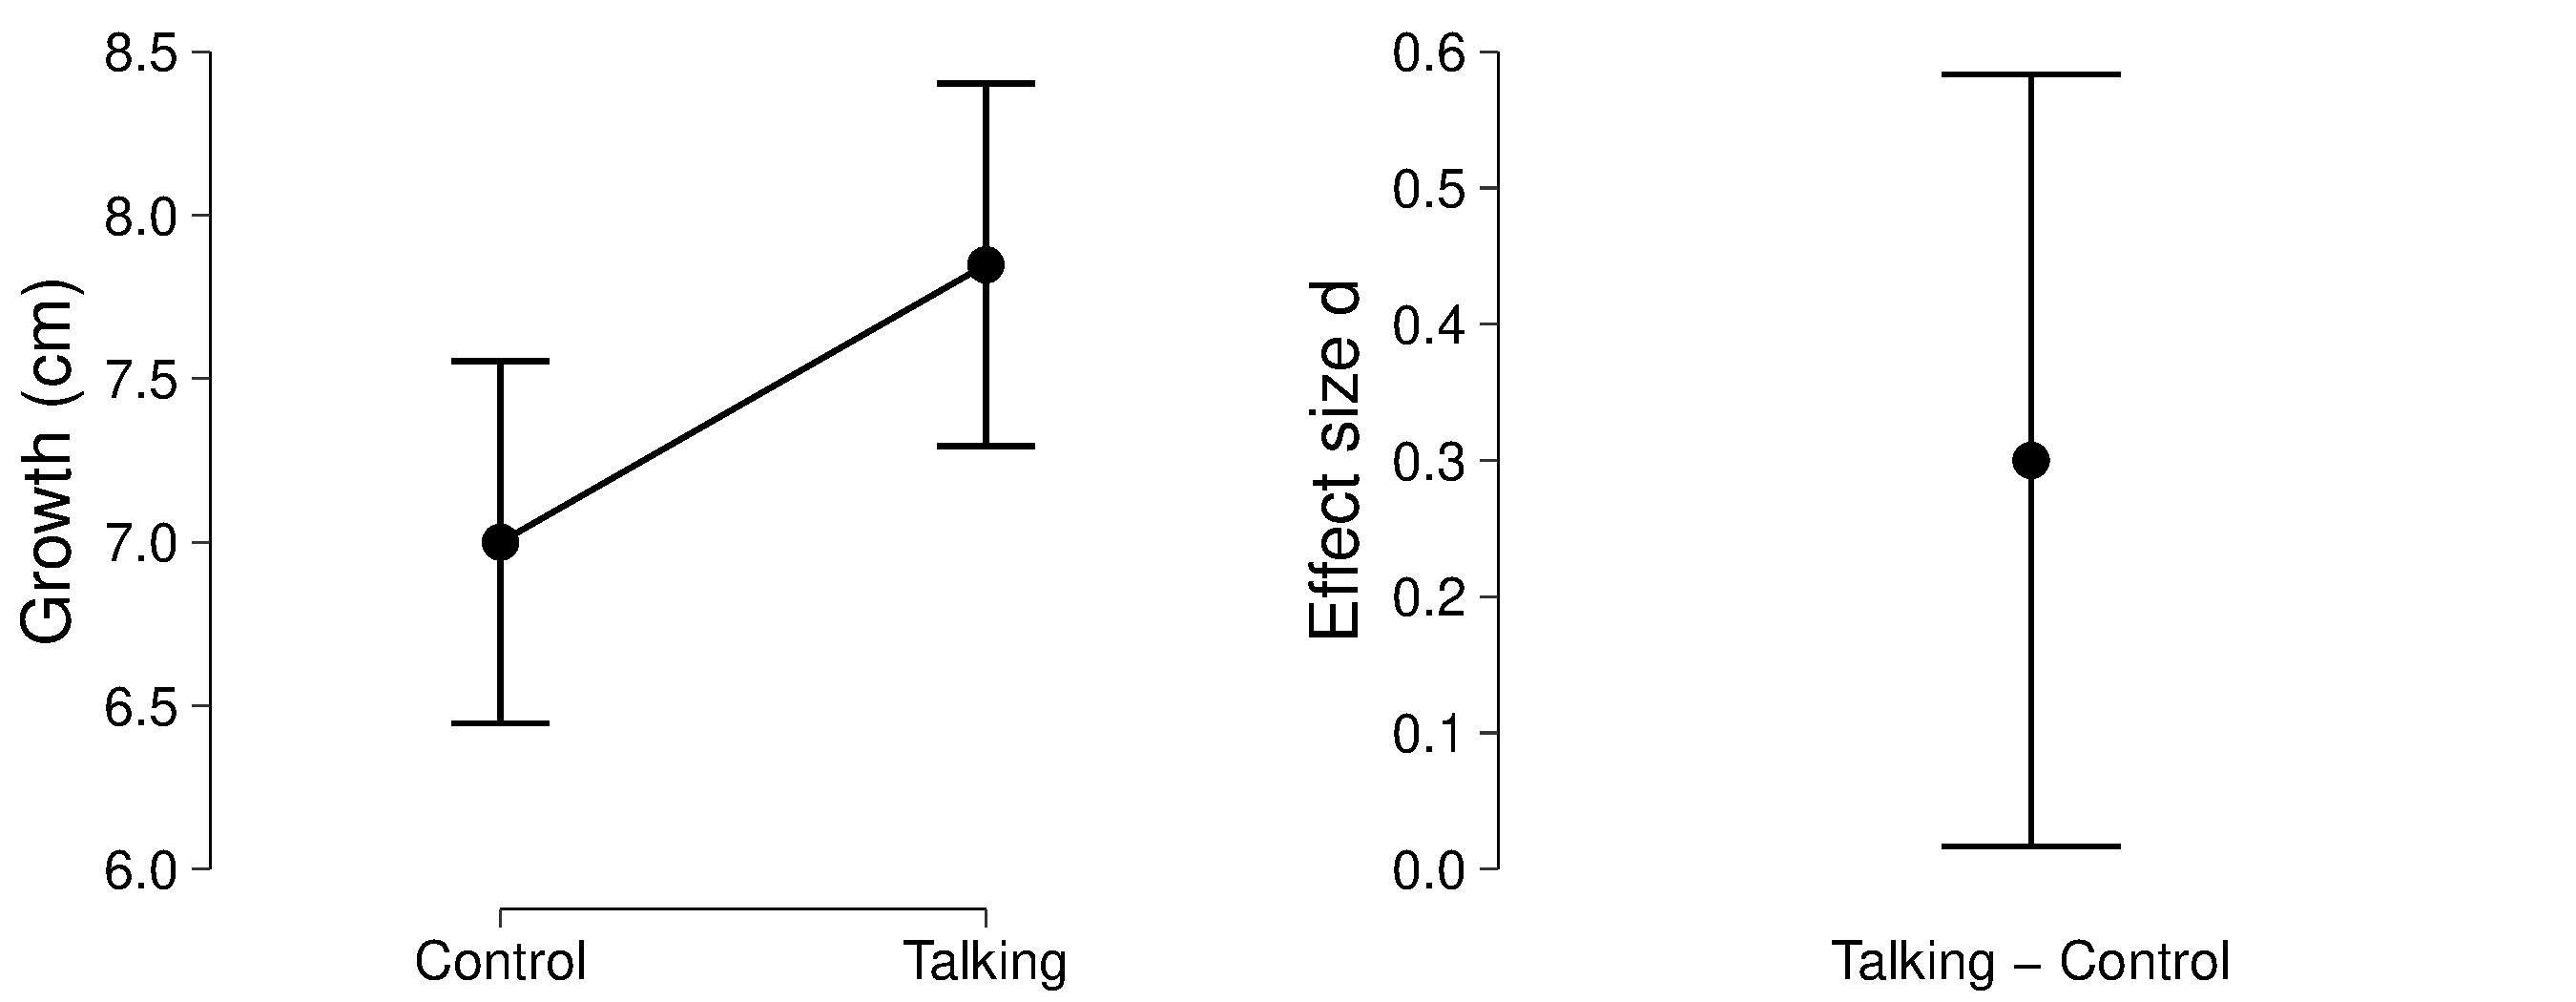
\includegraphics[width=\textwidth]{descriptivesPlot.pdf}
	\caption{Standard estimation results for the fictitious plant growth example. Left panel: a descriptives plot with the mean and 95\% confidence interval of plant growth in the two conditions. Right panel: point estimate and 95\% confidence interval for Cohen's \cohend.}
	\label{fig:descriptivesPlot}
\end{figure}


Based on these results, what would be a reasonable point estimate of effect size? A straightforward and intuitive answer is ``\getValue{0}{Estimate}{\tbEffectSizeExample}''. However, your colleague now informs you of the hypothesis that the experiment was designed to assess: ``plants grow faster when you talk to them''.%
\footnote{%
%Specifically, imagine your colleague selected 100 plants and weighted them three times: at the start of the experiment, after one week, and after two weeks.
%The first week 50 plants were randomly selected and spoken to, while the others served as controls.
%The next week the roles were reversed: the previously spoken to plants served as controls while the control plants were now spoken to.
%The quantity of interest is the difference in weight between the two conditions.
This example is inspired by \protect\textcite{BergerDelampady1987}.
} Suddenly, a population effect size of ``0'' appears eminently plausible. Any observed difference may merely be due to the inevitable sampling variability.%\footnote{\deleted{Unless your colleague talked out loud, with consumption, and the plants were near.}}

%\section*{\deleted{When Are Effect Sizes Overestimated?}}
\begin{revision}%
The example above is, of course, rhetorical.
In practice, hypotheses and expectations should be specified up front.
Nevertheless, the example raises the question: When are effect sizes overestimated?
\end{revision}%
Standard point estimates and confidence intervals ignore the possibility that the effect is spurious (i.e., the null hypothesis $\mathcal{H}_0$). This is not problematic when $\mathcal{H}_0$ is deeply implausible, either because $\mathcal{H}_0$ was highly unlikely \emph{a priori} or because the data decisively undercut $\mathcal{H}_0$. But when the data fail to undercut $\mathcal{H}_0$, or when $\mathcal{H}_0$ is highly likely \emph{a priori} (i.e., ``plants do not grow faster when you talk to them''), then $\mathcal{H}_0$ is not ruled out as a plausible account of the data. Effect size estimates that ignore a plausible $\mathcal{H}_0$ are generally \begin{revision}overly optimistic and\end{revision} overconfident: the fact that $\mathcal{H}_0$ provides an acceptable account of the data should shrink effect size estimates towards zero.
\begin{revision}%
For example, it is well known that the sample mean is not always the best estimator for the population mean but can be outperformed by shrinkage estimators \parencite{davis2018estimation, EfronMorris1977}.
\end{revision}
%\DON{It is well known that the sample mean is not always the best estimator (ref James Stein, Clint, Effron & Morris)}
%\begin{revision}%
%\DON{We could also briefly mention the spike-and-slab model here as a remedy to the problem introduced above.}
%\end{revision}%

\begin{revision}%
In this paper, we discuss the spike-and-slab model and its merits to avoid overestimating effect size.
First, we formally introduce the spike-and-slab model.
Second, we apply the spike-and-slab model to the example in the introduction and illustrate how it circumvents overestimation.
Third, we visualize how the spike-and-slab model may shrink the estimated effect size toward zero in general.
Fourth, we demonstrate the spike-and-slab model by reanalyzing the data of \textcite{heycke2018two}.
Finally, we conclude with practical recommendations and a discussion on when to use the spike-and-slab model.
\end{revision}


\section*{A Spike-and-Slab Perspective}
\begin{revision}%
The spike-and-slab approach has been broadly discussed in the statistical literature \parencite{ohara2009review, ishwaran2005spike, geweke1996variable} and psychological literature \parencite{yu2018bayesian, bainter2020improving}.
Conceptually, the approach is relatively straight-forward.
	
This section formalizes the conceptual ideas from the introduction in the spike-and-slab model \parencite{RouderEtAl2018PBR, clyde1996prediction, mitchell1988bayesian}. 
The population effect size is typically approximated with a sample estimate.
This sample estimate assumes that \hypo{0} is false and that the population effect size is nonzero.
To formalize this, let $\popDelta$ denote the population effect size, let $\obsDelta$ denote an estimate, and let $\obsDelta\mid\hypo{1}$ denote an estimate that assumes that \hypo{1} is true.
Assuming that \hypo{0} is true leads to $\obsDelta\mid\hypo{0}$, which is usually 0.
Key is that both estimates, $\obsDelta\mid\hypo{1}$ and $\obsDelta\mid\hypo{0}$, are \emph{conditional} on the hypotheses. 
For example, $\obsDelta\mid\hypo{1}$ should be read as ``the estimated effect size under the alternative hypothesis''.


%Such an estimate is denoted $\obsDelta\mid\hypo{1}$.
%Assuming that \hypo{0} is true, leads to an estimate denoted $\obsDelta\mid\hypo{0}$, which is usually 0. 
%Key is that both estimates, $\obsDelta\mid\hypo{1}$ and $\obsDelta\mid\hypo{0}$, are \emph{conditional} on the hypotheses. 
%For example, $\obsDelta\mid\hypo{1}$ should be read as ``the estimated effect size given that the alternative hypothesis is true''.
%Note that both estimates assume the hypothesis to be true; they ignore any uncertainty regarding the hypotheses themselves.
%The key property of the spike-and-slab model is that it considers both hypotheses at once in a two-component model. 
\end{revision}%
The first component\begin{revision}, the spike, \end{revision}corresponds to the position that talking to plants does not affect their growth (i.e., $\delta = 0$), whereas the second component\begin{revision}, the slab, \end{revision}corresponds to the position that speaking to plants does affect their growth (i.e., $\delta \neq 0$).
\begin{revision}%
\begin{revision}The spike and slab\end{revision} are analogous to \hypo{0} and \hypo{1} discussed above.
\end{revision}%
Both components are deemed \emph{a priori} equally likely, such that the prior probability for each component is \nicefrac{1}{2}.
\begin{revision}%
One can also assign prior probabilities other than \nicefrac{1}{2}, if this can be motivated by prior research or theories \parencite[e.g., ][]{wilson2018prior}.
After seeing the data, the prior probabilities of each component, $\prob{\shypo{0}}$ and $\prob{\shypo{1}}$, are updated to posterior probabilities, $\prob{\shypo{0}\mid\data}$ and $\prob{\shypo{1}\mid\data}$.

Quantifying the uncertainty about the two components using probabilities allows us to account for the uncertainty of each component.
Furthermore, this allows us to consider the \emph{marginal} estimate of effect size.
The marginal estimate of the spike-and-slab model weighs the estimates of each component by its plausibility after seeing the data.
That is, we sum the estimates conditional on each component weighed by the posterior probabilities of the components:
\begin{align*}
	\obsDelta = \left(\obsDelta\mid\shypo{0}\right)\prob{\shypo{0}\mid\data} + \left(\obsDelta\mid\shypo{1}\right)\prob{\shypo{1}\mid\data}.
\end{align*}

%To obtain the posterior probabilities, we need to choose an inferential paradigm.
The result is a \emph{marginal} estimate where the estimate of the slab is shrunken toward that of the spike (or vice versa).
To obtain a marginal estimate of effect size, we need to choose an inferential paradigm.
In a frequentist approach, one can use penalized maximum likelihood.
This foregoes marginalizing over the spike and slab and instead directly adds a penalty term to the likelihood to shrink estimates towards zero.
Well-known examples are LASSO and ridge regression \parencite{tibshirani2005sparsity}.
One frequentist approach that does marginalize uses information criteria to derive posterior probabilities for the spike and slab.
For example, take the Akaike Information Criterion \parencite[AIC;][]{Akaike1973} and define $\prob{\shypo{0}\mid\data} = \nicefrac{\AIC\mid\shypo{0}}{\left(\AIC\mid\shypo{0} + \AIC\mid\shypo{1}\right)}$.
This approach is taken by, for instance, \textcite{BurnhamAnderson2002}.

An alternative is a Bayesian approach.
Here we assign probability distributions to unknown parameters, such as effect size.
Even though choosing Bayesian analyses requires the specification of additional prior distributions, the advantage is that the posterior model probabilities follow directly from Bayes theorem.
Whereas frequentist approaches need to specify a penalty term or choose an information criterion, Bayesian approaches need to specify prior distributions on the model parameters (e.g., $\delta$) and the models themselves ($\prob{\shypo{0}}$ and $\prob{\shypo{1}}$).

%This requires us to specify additional prior distributions, however, the posterior model probabilities follow directly from Bayes theorem.% and do not depend on the choice of information criteria.
However, a Bayesian approach provides a posterior distribution for effect size which fully captures the uncertainty over possible effect sizes and allows for easy computation of uncertainty intervals.
In the remainder of this paper, we adopt the Bayesian approach for the spike-and-slab model.
For a full derivation of the posterior distribution, see Appendix A.%
\end{revision}

\begin{revision}To\end{revision} illustrate both the overestimation and \begin{revision}the spike-and-slab model we reanalyze\end{revision} the fictitious data from Figure~\ref{fig:descriptivesPlot}.
\begin{revision}%
	R code for the analysis is available at \osflink{}.
\end{revision}
In almost all current empirical work, an estimate of effect size is based solely on the \begin{revision}slab\end{revision}, which yields a point estimate and an uncertainty interval (for frequentists, $\obsDelta = \getValue{0}{Estimate}{\tbEffectSizeExample}$, 95\%  CI: \getCI{0}{\tbEffectSizeExample}; for Bayesians $\obsDelta = \getValue{1}{mean}{\reanalysis}$, 95\% CRI: \getCI{1}{\reanalysis}).
The spike-and-slab model, however, also considers the possibility that an effect can be absent; consequently, the overall estimate from the spike-and-slab model is a weighted average of the two components, shrinking the estimate towards zero.
Figure~\ref{fig:modelAveragedPosterior} contrasts the slab-only estimation against the spike-and-slab estimation.

\setValue{0}{ph1}{\reanalysis}{\phAlt}%
\setValue{0}{mode}{\reanalysis}{\modeAlt}%
\begin{figure}[!ht]
	\centering
	\begin{tikzpicture}
		\node[anchor=south west,inner sep=0] (image) at (0,0) {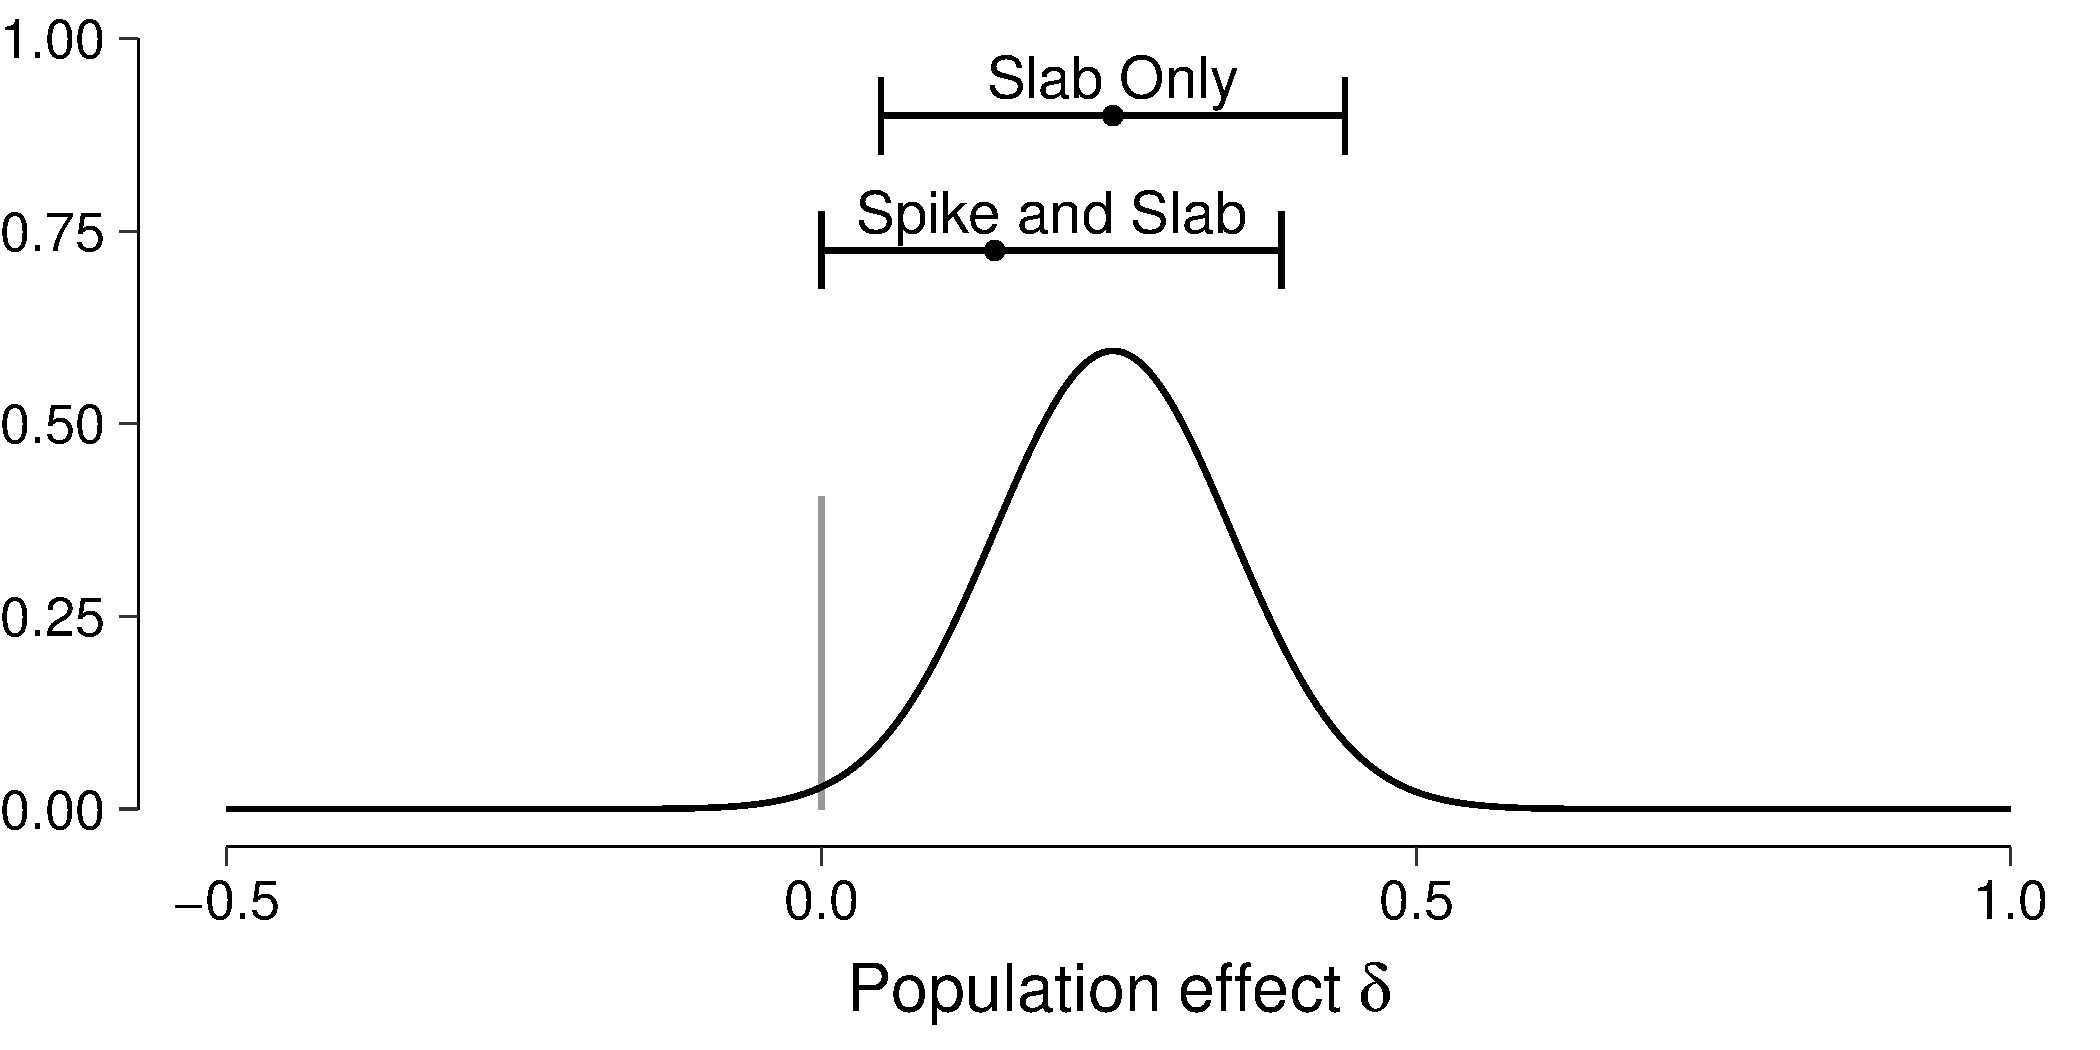
\includegraphics[width=0.9\textwidth]{spikeAndSlabPosteriorRescaledPosteriorMode.pdf}};
		\begin{scope}[x={(image.south east)},y={(image.north west)}]
		\node[anchor=base,inner sep=0pt, outer sep=0pt] at (0.28,0.62) {$p(\shypo{0}\mid\data) = \getValue{0}{ph0}{\reanalysis}$};
		\end{scope}
	\end{tikzpicture}
	\caption{
		The spike-and-slab model. The black line represents the posterior distribution of effect size given the slab (i.e., the effect is non-zero). The posterior is scaled so that its mode ($\obsDelta = \modeAlt$) equals the posterior probability of the alternative model (i.e., $p(\shypo{1}\mid\data) = \phAlt$). The grey line represents the posterior probability of the spike (i.e., $\obsDelta = 0$: the effect is absent). The error bars and dots above the density show 95\% credible intervals and the posterior mean for the slab-only model and for the spike-and-slab model.}
	\label{fig:modelAveragedPosterior}
\end{figure}
Compared to the traditional results based only on the slab, the posterior mean and central 95\% credible interval of the spike-and-slab model are shrunken towards 0 (i.e., \getValue{0}{mean}{\reanalysis} (95\% CRI: \getCI{0}{\reanalysis}) vs. \getValue{1}{mean}{\reanalysis} (95\% CRI: \getCI{1}{\reanalysis})). 
This shrinkage is due to the non-negligible probability that the effect is absent. 
The spike-and-slab posterior represents the plausibility that the effect is absent by the height of the spike, and the uncertainty about the effect's magnitude, given that it is present, by the width of the slab. 
Note that as the posterior probability of \begin{revision}the spike\end{revision} decreases, the spike-and-slab results approach those of the slab-only model.


\begin{revision}%
\section*{The Influence of the Spike}

In the fictitious example, the spike-and-slab model avoids overestimation by shrinking estimates of effect size towards zero.
That result may not be surprising, as the effect was small.
However, it makes one wonder to what extent the spike-and-slab model helps with estimation.
What differs between a slab only model and the spike-and slab?
In this section, we illustrate how the estimated effect size shrinks towards zero in general. 
We visualize the shrinkage as a function of the observed effect size, the prior on the standard deviation of effect size under the slab, the sample size, and the prior probability of the spike.
We chose these parameters because the posterior distribution is fully determined by these quantities (see Appendix A).

Figure~\ref{fig:S_vs_SS_4_panel} shows the relation between the observed effect size and the estimated effect size for the slab and for the spike-and-slab for 40 observations and 100 observations.
All plots show that a smaller prior standard deviation of the slab induces more shrinkage towards zero.
This makes sense as a small prior standard deviation implies there is more prior mass near the mean of the prior, which is zero.
The influence of the prior standard deviation is intrinsic to a Bayesian approach, but not to the spike-and-slab model.
Comparing the plots between the two columns illustrates the influence of the spike; whenever the observed effect size is near zero, the estimate is shrunken towards zero in the right column but not in the left column.
However, when the observed effect size is far from zero, there is little shrinkage.
\begin{figure}[!ht]
	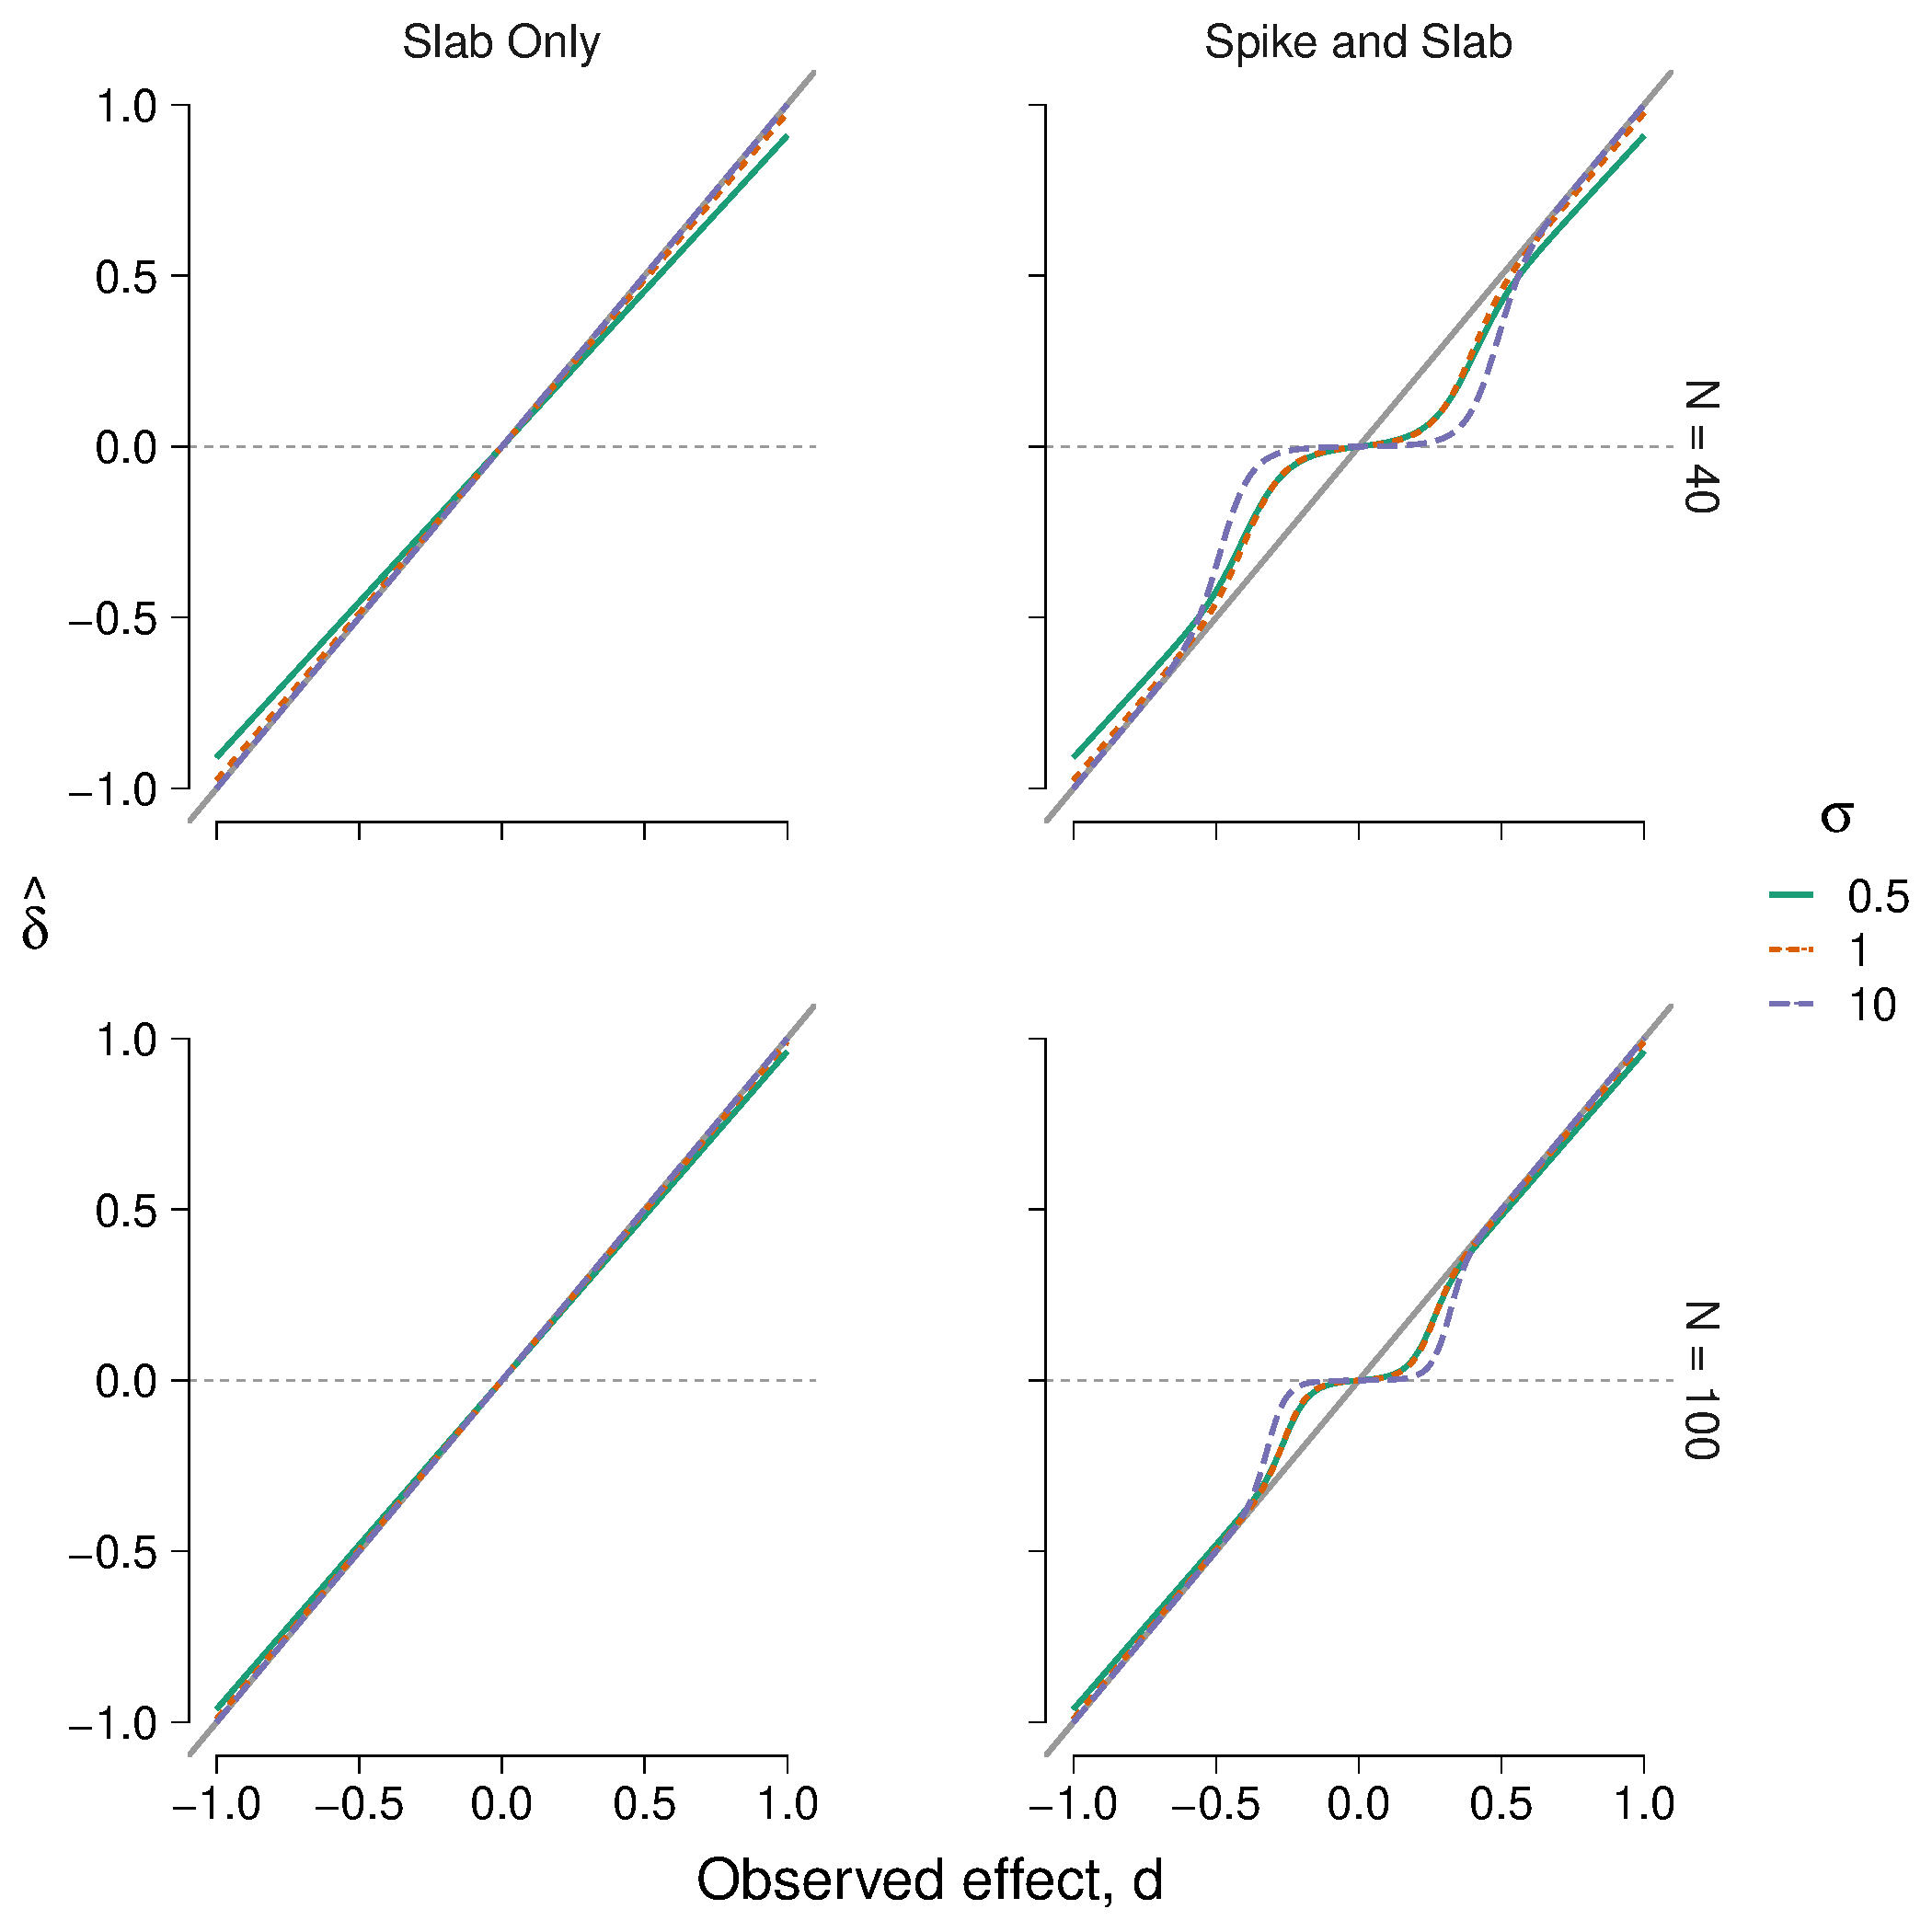
\includegraphics[width=\textwidth]{posteriorMeanVsSampleDelta_4_panel_big_font.pdf}
	\caption{%
		Observed effect size versus posterior mean for different model components and prior standard deviations.
		The left column shows inference based on the slab only model while the right column shows inference based on the spike-and-slab model.
		In the top row, the sample size was 40 while in the bottom row the sample size was 100.
		Different lines represent different standard deviations for the prior distribution on $\delta$.
		The prior probability of the spike was $\nicefrac{1}{2}$.
		Inspired by Figure~5 of \textcite{RouderEtAl2018PBR}.
	}
	\label{fig:S_vs_SS_4_panel}
\end{figure}
The shrinkage can be explained in the following way.
Whenever the observed effect size is small, the data are well described by an effect size of zero and thus the posterior probability of the spike is substantial.
As a result the marginal estimate is shrunken towards the spike's estimate, 0.
In contrast, when the observed effect size is large the data are poorly described by an effect size of zero and the posterior probability of the spike is negligible.
As a consequence, the estimate of the spike-and-slab is practically equivalent to the estimate of the slab.
The plots in the right column of Figure~\ref{fig:S_vs_SS_4_panel} shows the effect of sample size on the shrinkage.
For the bottom right plot, $N = 100$, if the observed effect size is small then the estimate is still shrunken towards 0, but as the observed effect size grows the shrinkage decreases much more quickly than in the top right plot where $N = 40$.
This makes sense from a signal-detection perspective. 
If the observed effect size is, for example, 0.3 after 40 observations, the posterior probability of the spike is substantial.
However, after collecting 60 additional observations while the observed effect size remains 0.3, the posterior probability of the spike decreases as it becomes increasingly less probable that the data generating model had an effect size of zero.


Next, we explore the relationship between shrinkage and the prior probability of the spike.
Figure~\ref{fig:S_vs_SS_PH0_40} shows the shrinkage for various prior probabilities.
The smaller the prior probability of the spike, the less the effect size is shrunken towards 0.
If the prior probability is small then the spike was a-priori implausible and less evidence is needed to make its influence negligible.
\begin{figure}[!ht]
	\centering
	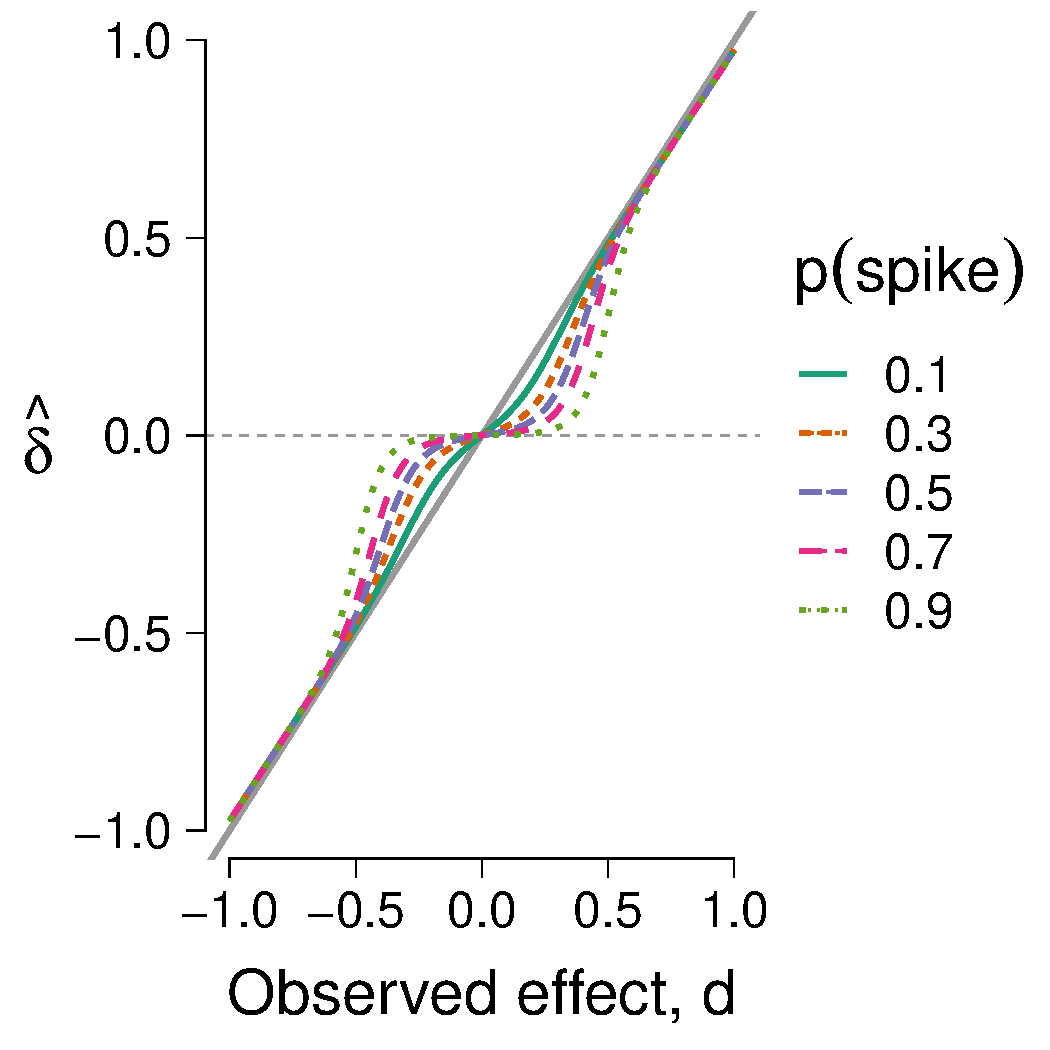
\includegraphics[width=.5\textwidth]{posteriorMeanVsSampleDelta_ph0_n_40_big_font.pdf}
	\caption{%
		Observed effect versus posterior mean (x-axis) versus the posterior mean of the spike-and-slab model (y-axis). The different lines represent different standard prior probabilities of the spike. The figure is based on 40 observations with a prior standard deviation of 1.
	}
	\label{fig:S_vs_SS_PH0_40}
\end{figure}

\section*{Empirical Example: Reanalysis of Two Minds}
To improve upon the previous fictional example, we highlight how the spike-and-slab approach can be used in psychological practice by reanalyzing the results of \textcite{heycke2018two}.
\textcite{heycke2018two} conducted two registered replications of \textcite{rydell2006two}.
We first briefly explain the design of the study before reanalyzing the results, for a detailed description see the ``Procedure'' section in \textcite{heycke2018two}. Afterward, we reanalyze the Explicit Evaluation and Implicit Evaluation analyses with a spike-and-slab model. Finally, we provide a robustness analysis.

Participants were shown a positive or negative prime on a computer screen followed by an image of a person.
Next, several behavioral descriptions that were either negative or positive appeared underneath the image of the person.
Participants were asked to indicate whether the behavioral description was characteristic or uncharacteristic for the person shown.
After the first block of trials, participants explicitly evaluated the target person and performed an implicit association task (IAT). 
In total, data of 51 participants was analyzed.
\textcite{heycke2018two} found that an explicit description had an effect while the IAT showed an indication of an effect.

\paragraph{Explicit Evaluation}
In the analysis of the explicit evaluations, \textcite[p.~10;][]{heycke2018two} conducted a paired t-test and concluded that the rating of the target character is more positive if positive information is shown before negative information: $t(27) = 11.52$, $p < .001$; $\mathrm{BF}_{10} = 1.37\times10^9$, $d = 2.09$, 95\% HDI $[1.41, 2.79]$.%
\footnote{%
These are the statistics reported by \textcite{heycke2018two}.
BF stands for Bayes factor, see also appendix A. HDI is short for highest density interval, a type of credible interval.
}
The magnitude of the effect is large and thus a spike-and-slab reanalysis yields practically the same results: $\obsDelta = \getValue{0}{modelAveraged}{\reanalysisHeycke}$, 95\% CRI: \getCI{0}{\reanalysisHeycke}.%
\footnote{%
The difference between the point estimate and the credible intervals is possibly caused by the difference in prior distributions for effect size. 
\textcite{heycke2018two} use a Cauchy prior whereas we use a normal prior.% sqrt(2)/2
}

\paragraph{Implicit Evaluation}
In the analysis of the IAT, \textcite[p.~10;][]{heycke2018two} conducted a paired t-test and concluded that when negative primes were presented before positive primes there was some indication that the IAT rating became more negative: $t(27) = -2.54$, $p = .017$, $\mathrm{BF}_{10} = 2.92$, $d = -0.44$, 95\% HDI $[-0.83, -0.06]$.
Here, the magnitude of the effect is smaller and as a consequence the results from the spike-and-slab reanalysis are more conservative: $\obsDelta = \getValue{1}{modelAveraged}{\reanalysisHeycke}$, 95\% CRI: \getCI{1}{\reanalysisHeycke}.
The estimate of effect size is shrunken towards 0 because the spike provides a reasonable account of the data,  $\prob{\shypo{0}\mid\data} = \getValue{1}{ph0}{\reanalysisHeycke}$.

\paragraph{Robustness analysis}
In the reanalyses above the prior probability of the spike was set to 0.5. One might wonder how robust or how volatile the results are to changes in the prior probability of the spike.
\begin{figure}[!ht]
	\centering
	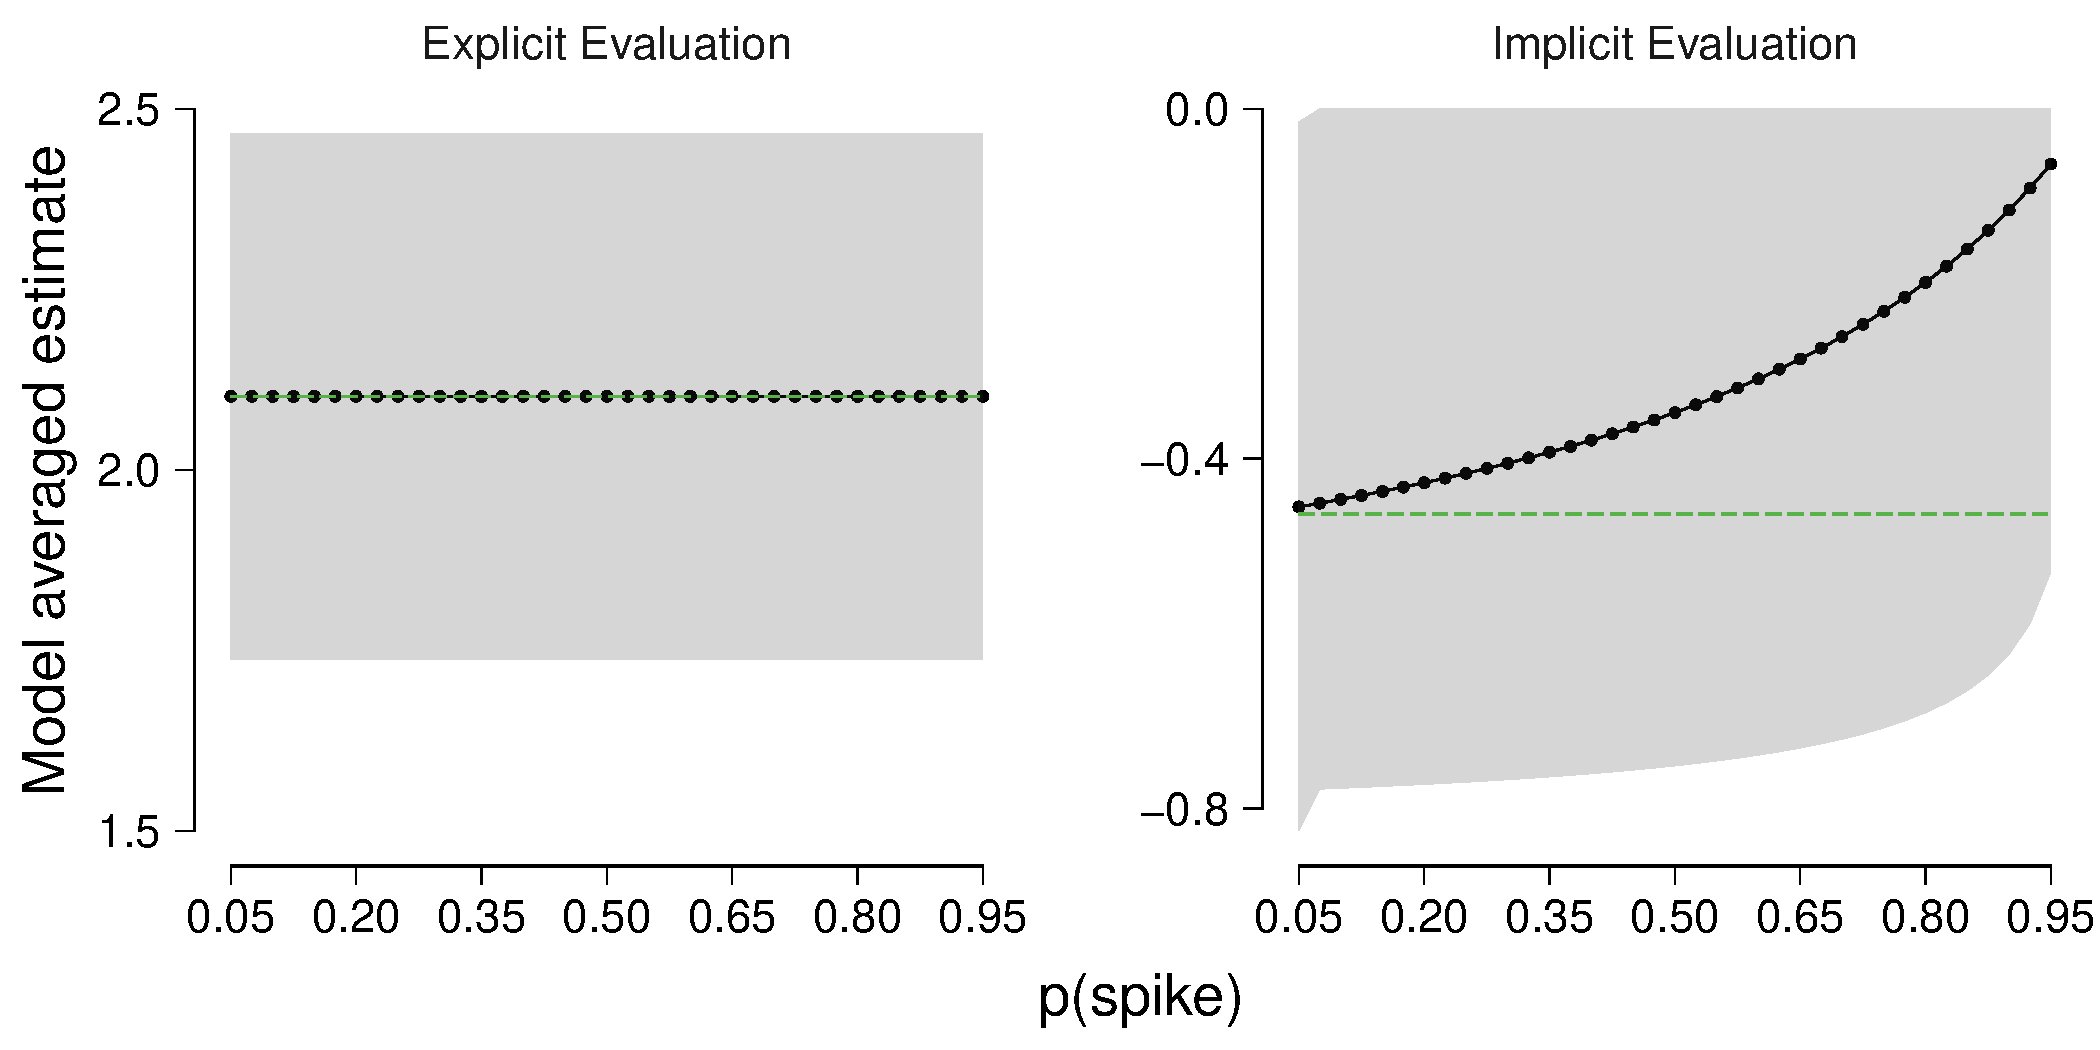
\includegraphics[width=\textwidth]{robustnessReanalysis_big_font.pdf}
	\caption{%
		Robustness analysis that shows the prior probability of the spike (x-axis) versus spike-and-slab estimates (y-axis) for the explicit evaluation (left~panel) and the implicit evaluation (right panel).
		Solid points show the point estimate of the spike-and-slab and the gray area represents the accompanying 95\% credible interval.
		The green horizontal dashed line shows the estimate of the slab.
	}
	\label{fig:robustnessReanalysis}
\end{figure}
Figure~\ref{fig:robustnessReanalysis} visualizes the influence of the prior on the spike. 
In the left panel that shows the explicit evaluation data, the different estimates for different prior probabilities are practically identical. 
For this analysis, the data dominate the prior.
In contrast, in the right panel that shows the explicit evaluation data, the prior probability of the spike has a large impact on the results.
Here, the data are less informative and the prior has more influence.
The adaptive shrinkage is a key feature of the spike-and-slab, that is, the amount of shrinkage depends on the posterior plausibility of the spike.
\end{revision}


\section*{Discussion}
Standard estimates of effect size ignore the null hypothesis and are therefore overconfident, that is, \begin{revision}farther\end{revision} from zero \begin{revision}than they should be\end{revision}. The spike-and-slab model remedies this problem by explicitly considering the possibility that an effect is absent \parencite{Robinson2019,RouderEtAl2018PBR}. The core idea dates back to
\citeauthor{Jeffreys1939} (\citeyear{Jeffreys1939}; see also \citeauthor{ly2020bayesian}, \citeyear{ly2020bayesian}); nonetheless, it is \begin{revision}largely\end{revision} ignored in empirical practice, in statistical education, and in journal guidelines.
\begin{revision}%
We believe the spike-and-slab model is a useful addition to existing statistical tools of researchers and that it will make the interpretation of the estimates, even those from a preregistered study, more robust across different models.
\end{revision}

\subsubsection*{What if All Null Hypotheses Are False?}
The spike-and-slab approach clashes with the popular estimation mindset, where it is argued that statistical significance should be abandoned in favor of estimation \parencite{McShane2019abandon, Cumming2016introduction, valentine2015life, Cumming2014}. 
One argument to forgo hypothesis testing is that all null hypotheses are false \parencite{Cohen1990, Meehl1978} and therefore there is no need to consider a component that states that an effect is exactly zero. 
The statistical counterargument is that, even if point null hypotheses are false, they are still mathematically convenient approximations to more complex hypotheses that allow mass on an interval close to zero \parencite[\begin{revision}i.e., perinull hypotheses;\end{revision}][]{ly2020bayesian2, george1993variable, BergerDelampady1987}. 
Thus, from a pragmatic perspective it is irrelevant whether or not null hypotheses are exactly true: in the spike-and-slab model, a \begin{revision}narrow interval around zero\end{revision} will shrink estimates towards zero almost as much as the point null spike component will. 

\subsubsection*{When to Ignore the Spike}
There are two scenarios in which the presence of the spike can safely be ignored.
First, the spike may be deeply implausible.
This happens most often in problems of pure estimation, such as when determining the relative popularity of two politicians or the proportion of Japanese cars on the streets of New York.
In such cases, no value or interval needs to be singled out for special attention.
Second, the data\begin{revision}, or data from prior studies,\end{revision} may provide overwhelming evidence that an effect is present\begin{revision}, as in the reanalysis of the Explicit Evaluation data.\end{revision}
When this happens, the results from a spike-and-slab model become virtually identical to those of a slab-only model, and the inclusion of the spike does not offer an added benefit albeit that the spike also does not hurt. %A practical recommendation by Harold Jeffreys is to ignore the spike whenever sample sizes fall between 50 and 2000 and the maximum likelihood estimate deviates from the spike by more than three standard errors (\cite[pp. 193--194]{Jeffreys1939}; \cite[p. 75]{Jeffreys1980}).



\subsubsection*{Conclusion}
Standard methods for estimating effect size produce results that are overly optimistic.
This \begin{revision}tendency\end{revision} toward high estimates can be corrected by applying the spike-and-slab model which explicitly accounts for the possibility that the effect is absent. 
\begin{revision}%
%%The spike-and-slab approach is not meant as a *gotcha* method to reanalyze other researchers' data that one does not believe in.
The spike-and-slab approach is not meant as a tool to downplay other researchers' findings that one does not believe in.
Instead, it provides a more robust estimate of the size of an effect of high-quality studies if null and alternative hypothesis are plausible.
We believe that approach allows researchers a more nuanced interpretation of their own results taking into account the plausibility that there is any effect.
\end{revision}

%\newpage
\printbibliography

\newpage
\appendix
\begin{revision}%

\section*{A: Derivation of the Posterior Distribution}

%\DON{mention in the cover letter that this can also be an online appendix}

Here we derive the posterior distribution for the spike-and-slab model. We first derive the results for the slab and spike individually and afterward we combine them. Using the slab, we explain the model and assign a prior distribution to effect size. Afterward, we use Bayes' theorem to obtain the posterior distribution for the parameters.

In the example, we use a paired samples t-test. Following \textcite{RouderEtAl2018PBR}, we assume that the differences between the paired samples, denoted $\dataZi$, are normally distributed with unknown mean $\delta$ and a known variance of $1$.
As prior distribution for $\delta$ we use a normal distribution with mean 0 and unknown variance $\sigma^2$.
This implies $\dataZi\sim \dnorm{\delta}{1}$ for the data and $\delta\sim\dnorm{0}{\sigma^2}$ for the prior. The posterior distribution for $\delta$ is obtained through Bayes' theorem:
\begin{align*}%\label{eq:BayesTheorem2}
\overbrace{\probp{\delta \mid \dataZ}}^{\substack{\text{Posterior}\\\text{distribution}}}
= 
%\overbrace{\probp{\bm{\model}}}^{\substack{\text{Prior model}\\ \text{probability}}}
%\times	\quad
\overbrace{\probp{\delta}}^{\substack{\text{Prior}\\ \text{distribution}}}
\times \quad
\frac{
	\overbrace{\lik(\dataZ \mid \delta)}^{\text{Likelihood}}
}{
%	\probp{\data}
	\underbrace{\probp{\dataZ}}_{\substack{\text{Marginal}\\ \text{Likelihood}}}
}.
\end{align*}
For the prior distribution we use a normal distribution with mean 0 and variance $\sigma^2$. The likelihood is given by:
\begin{align*}
	\lik(\dataZ \mid \delta, \shypo{1}) &= \prod_{i=1}^{N} \dnormc{\dataZi}{\delta}{1},\\
							 &= \left(2\pi\right)^{-\frac{N}{2}}
							 \exp\left(-\frac{N}{2}\left(\meanZ + \varZ + \delta^2 -2\meanZ\delta\right)\right),
\end{align*}
where $\meanZ$ and $\varZ$ are the sample mean and sample variance of $\dataZi$ respectively. Next, we compute the marginal likelihood by integrating out the likelihood times prior with respect to $\delta$.

\begin{align*}
	\probp{\dataZ\mid\shypo{1}} &=\int_{-\infty}^{\infty} \lik(\dataZ \mid \delta) \probp{\dataZ} 	\dx{\delta},\\
%	&= 
%	\left(2\pi\right)^{-\frac{N+1}{2}}
%	\exp\left(-\frac{N}{2}\left(\meanZ + \varZ\right)\right) \\
%	&\times\int_{-\infty}^{\infty}
%	\exp\left(-\frac{N}{2}\left(\delta^2 -2\meanZ\delta\right)\right)
%	\exp\left(-\frac{1}{2\sigma^2}\delta^2\right)
%	\dx{\delta},\\
	&=\left(2\pi\right)^{-\frac{N+1}{2}}
	\exp\left(-\frac{N}{2}\left(\meanZ + \varZ\right)\right), \\
	&\times\int_{-\infty}^{\infty}
	\exp\left(-\frac{1}{2}\left(\delta^2\left(N + \frac{1}{\sigma^2}\right) -\delta \frac{2N\meanZ}{\sigma^2}\right)\right)
	\dx{\delta}.
\end{align*}
Here we may recognize a Gaussian integral and use the following identity:
\begin{align*}
	\int_{-\infty}^{\infty}\exp\left(-ax^2+bx+c\right)\dx{x} &= \sqrt{\frac{\pi}{a}}\exp\left(\frac{b^2}{4a}+c\right).
\end{align*}
Filling in the identity and simplifying yields:
\begin{align*}
	\probp{\dataZ\mid\shypo{1}} &= 	
	\left(2\pi\right)^{-\frac{N}{2}}
	\exp\left(-\frac{N}{2}\left(\meanZ + \varZ\right)\right)
	\frac{
		\exp\left(\frac{N^2 \meanZ^2}{2\left(N+\frac{1}{\sigma^2}\right)}\right)
	}{
		\sqrt{N+\frac{1}{\sigma^2}}
	}.
\end{align*}

Next, we can obtain an expression for the posterior distribution. However, often it suffices to write out the expression for the likelihood times prior and then (somehow) recognize a known distribution. This is particularly common in Gibbs sampling where one is interested in the conditional posterior distributions. We also do this here, as it reduces inference about the posterior distribution (e.g., what is the mean or variance) to inference about a known distribution, in this case a normal distribution:
\begin{align*}
	\probp{\delta \mid \dataZ, \shypo{1}} &\propto  
	\left(2\pi\right)^{-\frac{N}{2}}
	\exp\left(-\frac{N}{2}\left(\meanZ + \varZ\right)\right) 
	\exp\left(-\frac{N}{2}\left(\delta^2 -2\meanZ\delta\right)\right),\\
	&\times \left(2\pi\right)^{-\frac{1}{2}} \exp\left(-\frac{1}{2\sigma^2}\delta^2\right), \\
	&\propto 
	\exp\left(-\frac{1}{2}\left(\delta^2\left(N + \frac{1}{\sigma^2}\right) -\delta \frac{2N\meanZ}{\sigma^2}\right)\right).
\end{align*}
We recognize a normal distribution with variance $\sigma_1^2 = \frac{1}{N + \frac{1}{\sigma^2}}$ and mean $\mu_1 = N\meanZ\sigma_1^2$. Thus we have $\probp{\delta \mid \dataZ} \propto \dnorm{\mu_1}{\sigma_1^2}$.

Next we compute the same for the spike. The spike states that $\dataZi\sim \dnorm{0}{1}$ and contains no parameters to estimate. Thus there are no prior distributions to specify and the only thing we need to compute is the marginal likelihood:
\begin{align*}
	\probp{\dataZ\mid\shypo{0}} &= 
	\left(2\pi\right)^{-\frac{N}{2}}
	\exp\left(-\frac{N}{2}\left(\meanZ + \varZ\right)\right).
\end{align*}
Using both marginal likelihoods we can now obtain the Bayes factor in favor of the spike:
\begin{align*}
	\text{BF}_{01} &= \frac{\probp{\dataZ\mid\shypo{0}}}{\probp{\dataZ\mid\shypo{1}}} =
	\frac{
		\sqrt{N+\frac{1}{\sigma^2}}
	}{
		\exp\left(\frac{N^2 \meanZ^2}{2\left(N+\frac{1}{\sigma^2}\right)}\right)		
	}.
\end{align*}
We may now obtain inference for both the spike and the slab by computing the posterior probability of the slab:
\begin{align*}
	\prob{\shypo{1}\mid \dataZ} &= \frac{\prob{\shypo{0}}}{\prob{\shypo{0}} + (1 - \prob{\shypo{0}})\text{BF}_{01}}.
\end{align*}
It follows that the cumulative distribution function for the spike-and-slab posterior is given by:
\begin{align*}
	P(\delta\leq x \mid \dataZ) =
	\begin{cases}
	\prob{\shypo{1}\mid \dataZ}\Phi(x;\mu_1,\sigma_1)	 							& \text{if $x < 0$,} \\
	\prob{\shypo{0}\mid \dataZ} + \prob{\shypo{1}\mid \dataZ}\Phi(x;\mu_1,\sigma_1)	& \text{if $x \geq 0$,}\\
	\end{cases}
\end{align*}
where $\Phi(x;\mu_1,\sigma_1)$ is the cumulative normal distribution. Due to the discontinuity at $x = 0$ there is no useful closed form expression for the posterior density. Nevertheless, the posterior mean of the spike-and-slab model is available in closed form. Using the law of total probability, we have: 
\begin{align*}
	p(\delta\mid \dataZ) &= \prob{\shypo{0}\mid \dataZ}p(\delta\mid\shypo{0}, \dataZ) + \prob{\shypo{1}\mid \dataZ}p(\delta\mid\shypo{1}, \dataZ).
\end{align*}
Computing the mean of left hand side yields:
\begin{align*}
	\int_{-\infty}^\infty \delta \, p(\delta\mid \dataZ) \dx{\delta} &= 
	\prob{\shypo{0}\mid \dataZ}\int_{-\infty}^\infty\delta \, p(\delta\mid\shypo{0}, \dataZ) \dx{\delta}, \\
	&+ \prob{\shypo{1}\mid \dataZ}\int_{-\infty}^\infty\delta \, p(\delta\mid\shypo{1}, \dataZ) \dx{\delta}, \\
	&=
	0 + 
	\prob{\shypo{1}\mid \dataZ} \left(\mu_{\delta} \mid\shypo{1}, \dataZ\right).
\end{align*}
Here $\left(\mu_{\delta} \mid\shypo{1}, \dataZ\right)$ is the posterior mean of effect size under the slab. In a similar fashion, other statistics may be obtained. However, it is also possible to draw samples from marginal posterior distribution. To obtain a sample $s$, first draw $u$ from a uniform distribution on [0, 1]. If $u<\prob{\shypo{1}\mid \dataZ}$ draw $s$ from $p(\delta\mid\shypo{1}, \dataZ)$, otherwise $s$ is zero. This approach often used when the integrals become too unwieldy to compute analytically. For example, the R package BAS uses this procedure to compute credible intervals \parencite{ClydeEtAl2011}.

\end{revision}

\end{document}